\section{Analytical Modeling}
In the previous section we studied the possibility of using a polynomial to capture the relationship between grain size, number of cores, and throughput for a fixed matrix size, with the purpose of finding a range of grain size that leads us to maximum performance. 
Although the polynomial function was helpful in directing us toward our objective, it does not have a physical implication. 

This motivated us to change our view, and instead of looking just at the data and trying to find a function to fit the data, study the behavior of the data, and then find a function that would be likely to fit the data. That function would be a good fit mostly because that's how we expect the throughput to change with grain size, and not just how the data looks like.   

In this chapter we attempt to understand the effect of grain size on the achievable speedup in an asynchronous many-task runtime system. As discussed in chapter~\ref{Background}, our knowledge here comes from Amdahl's law and Universal Scalibility Law, which is an extension to the Amdahl's law. What these models suggest is that as we increase the number of cores in a multicore system, we do not observe a linear speedup, and they hold two major factors accountable for that, latency.

Here we are interested in developing an analytical model for predicting the execution time in an asynchronous many task runtime system. Even if we were able to determine all the factors affecting the execution time, it is still very hard to find an analytical model describing the relationship between these factors and the execution time.   

Definitions:
We represent the overhead of creating one task with $\alpha$, the number of tasks created with $num\_{tasks}$, the maximum amount of work assigned to one core as $w\_c$, the number of cores that are actually doing the work as $M$, the total amount of work available as $problem\_{size}$, and the sequential execution time as $t_{seq}$.

In an attempt to find this analytical model, we started with looking into two major factors, the overhead of creating tasks, and the maximum amount of work assigned to one core. 
In order to understand how these factors contribute to the execution time, we created a benchmark based on a simple \textit{for\textunderscore{loop}} with different number of iterations, iteration lengths, and chunk sizes, as shown in Listing~\ref{hpx_for_loop}. 
Each iteration consists of a while loop that makes sure the iteration lasts a certain amount ot time. This way, knowing how long it would take to execute one iteration(denoted as \textit{iter\textunderscore{length}}), how many of iterations are executed by one HPX thread(denoted as \textit{chunk\textunderscore{size}}), and finally how many iterations there are(denoted as \textit{num\textunderscore{iterations}})), we can see how the execution time changes when the problem is executed on different number of cores. Here, we define \textit{problem\textunderscore{size}} as the time it takes to execute all the iterations, which is:

\begin{equation}\label{problem_size}
problem\_size = iter\_length\times{num\_iterations}
\end{equation}

The total execution time could be assumed to be the maximum amount of time it takes for one of the cores to finish it's work. With this assumption, the execution time for this simple problem, could be estimated as summation of maximum overhead of creating tasks on one core, the overhead of managing the tasks created on one core, and the time it takes to run $w\_c$ amount of work when $M$ cores are available, shown in Formula~\ref{formula1}. 

While the overhead of creating a task should be constant on a specific machine architecture, we are suggesting here that the overall overhead of managing $num\_{tasks}$ tasks, is a factor($\delta$) of $N$. This effect is originated from HPX's strategy to avoid allocating new stacks by keeping the previous stack alive until new thread is created, at this point the stack is assigned to the new thread. 

%On the other hand, when number of tasks created is smaller than the number of cores, we observe continuous efforts from the idle cores to steal work from cores that are actually doing the work, interrupting the cache coherency constantly. We represent this effect with $\delta\times{(N-M)\times{M}}\times{num\_{tasks}}\times{\frac{1}{M}})$.


We represent the overhead of creating a task on a machine with $\alpha$, and the overhead of managing a task on a machine with $\delta\times\frac{{N}\times{num\_{tasks}}}{N}=\delta\times{num\_{tasks}}$. 

Looking at the execution time as the maximum amount of execution time among all the cores, we can formulate the execution time as:  

\begin{equation}\label{formula1}
\begin{aligned}
&execution\_time = \\
&\left\{
\begin{aligned}
&
\alpha\left\lceil{\frac{num\_{tasks}}{M}}\right \rceil +\delta\times{num\_{tasks}}+{w\_c+\gamma\times{w\_c}\times{(M-1)}} \:\: \text{if\:\:}num\_{tasks}>N\\
&\alpha\left \lceil{\frac{num\_{tasks}}{M}}\right \rceil +\delta\times{(N-num\_{tasks})}\times{num\_{tasks}}+{w\_c+\gamma\times{w\_c}\times{(M-1)}} \:\: \text{otherwise}
\end{aligned}
\right.
\end{aligned}
\end{equation}

%\begin{equation}\label{formula1}
%\begin{aligned}
%&execution\_time = \\
%\left\{
%\begin{aligned}
%&
%\alpha\left\lceil{\frac{num\_{tasks}}{M}}\right \rceil +\beta\times{(N-1)}{num\_{tasks}}+{w\_c+\gamma\times{w\_c}\times{(M-1)}} \:\: \text{if\:\:}num\_{tasks}>N\\
%&\alpha\left \lceil{\frac{num\_{tasks}}{M}}\right \rceil +\delta\times\frac{num\_{tasks}-1}{N}+{w\_c+\gamma\times{w\_c}\times{(M-1)}} \:\: \text{otherwise}
%\end{aligned}
%\right.
%\end{aligned}
%\end{equation}
%\vspace{\baselineskip}

Where, 
\begin{equation}\label{formula2}
w\_c =\left\{
\begin{aligned}
&problem\_{size} \:\:\:\:\:\:\:\:\:\:\:\:\:\:\:\:        \text{ if } N=1\\
&problem\_{size}-g\times{(N-1)}\times(\left \lceil{\frac{num\_{tasks}}{N}}\right \rceil-1)
 \text{if }num\_{tasks}\%N=1\text{\:\:and\:\: }num\_{iterations}\%chunk\_{size}\neq0\\ 
%\text{\:\:or} \\ g\times(\left \lceil{\frac{num\_{tasks}}{M}}\right \rceil-1)+(num\_{iterations}\%chunk\_{size})\times(iter\_{length}) \\ \:\:\:\:\:\:\:\:       
&g\times\left \lceil{\frac{num\_{tasks}}{N}}\right \rceil  \:\:\:\:\:\:\:\:       \text{otherwise}
\end{aligned}
\right.
\end{equation}

The first and second part of Formula~\ref{formula1} is associated with the overhead of creating and managing $num\_{tasks}$ tasks on $N$ cores, while considering the effect of work stealing ,and the last part is deducted from the Universal Scalibilty Law\cite{gunther2007guerrilla}, that suggests an overhead associated with the number of cores should be added to the expected execution time. Here, we adjusted the total number of cores ($N$) to the number of cores that are actually executing the work ($M$). 

Assuming we are running our application on $N$ cores, with a grain size equal to $g$, $num\_{tasks}$ tasks are being created, and $M$ cores are actually doing the work. If $num\_{tasks}<N$, $M$ would be equal to $num\_{tasks}$, otherwise $M=N$.

\begin{equation}\label{formula19}
M=\left\{
\begin{aligned}
num\_{tasks} \text{\:\:\:\:if \:} num\_{tasks}<N\\
N \text{\:\:\:\:otherwise}
\end{aligned}
\right.
\end{equation}

Figure shows an example of the results obtained from running the benchmark, for $problem\_size=10000$, on different number of cores.

\vspace{\baselineskip}	
\begin{figure}[H]
	\centering
	{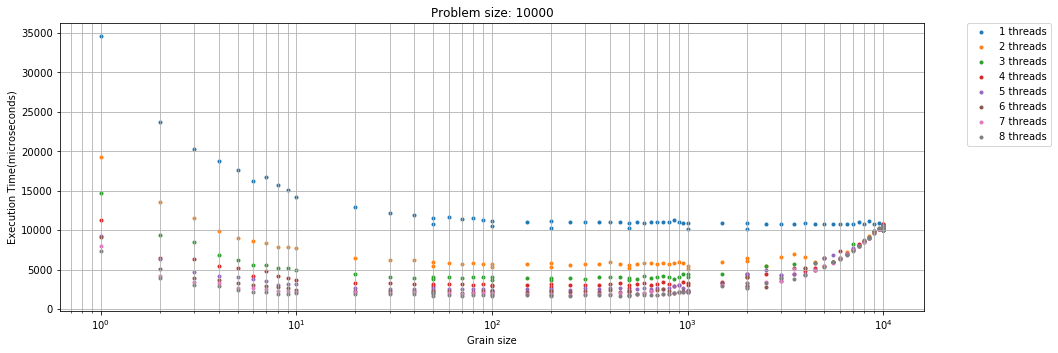
\includegraphics[scale=.45]{images/hpx_for_loop/10000_8_all.png}}
	\caption{The results of running the benchmark in Listing with $problem\_size=10000$, on different number of cores.}\label{fig39}		
\end{figure}

As stated in Chapter~\ref{Background}, at the right hand side of the graph in Figure~\ref{fig39}, the number of tasks created is smaller than the number of cores which results in making at least one of the cores idle, while the other cores are assigned a rather big chunk of work. The performance degradation we observe in that points is associated with starvation, meaning that we are not utilizing our computation resources to the full extent. In these points, the number of cores actually doing the work is equal to the number of the tasks, since each core gets to execute at most one task. At this region of the graph, the maximum assigned work to a core ($w\_c$) is the dominant factor.   

On the other hand, on the left hand side of the graph, since the grain size is very small we end up with creating a large number of tasks. Since there is an overhead associated with each created task, we observe a performance degradation in that region. As the grain size increases, the number of created tasks, and the overhead associated to that decreases consequently. At this region of the graph, the overhead of creating the tasks($\alpha\times{num\_{tasks}}$) is the dominant factor.   





From overhead point of view though, if we represent the overhead of creating one task on a particular machine as $\alpha$, the overhead of creating $num\_{tasks}$ tasks would be $\alpha\times{num\_{tasks}}$, but this overhead is divided between the $M$ cores actually doing the work. 

To summarize, for this simple experiment, where we do not have to deal with the cash effects, we believe the important factors are: number of HPX threads being created, number of cores the program is ran on, the maximum amount of work one core has to perform. The maximum number of tasks assigned to one core, and the number of cores that are actually performing the work, are two other important factors that can be deducted from the aforementioned factors. 

\vspace{\baselineskip}
\subsection{Analyzing the Data}
Assuming the proposed formula is a good fit for this problem, we can estimate the range of grain sizes for which we achieve the lowest execution time, for a specific problem size, run on specific number of cores.

\vspace{\baselineskip}
\subsubsection{Left side of the graph}
As stated earlier, in Formula~\ref{formula1}, for small grain sizes the first term is the dominant factor while the second term roughly stays constant. Same way, for large grain sizes the second factor is the dominant factor. 

In order to find the lower-bound of the range for which the execution time stays constant, we assume the second factor is constant in that region. Also we can change $N$ to $M$, knowing that our concern is on the left hand side of the graph, where $num\_{tasks}$ is definitely greater than the number of cores. 
Taking the derivative of the function based on the grain size then leads to:

 
\begin{equation}\label{formula3}
\begin{aligned}
\frac{\partial execution\_{time}}{\partial g} &= \frac{\alpha}{N}\times{\frac{\partial num\_{tasks}}{\partial g}}+\beta\times(N-1)\times{\frac{\partial num\_{tasks}}{\partial g}} \\
&=(\frac{\alpha}{N}+\beta\times(N-1))\times\frac{\partial(\frac{problem\_{size}}{g})}{\partial g} \\
&=(\frac{\alpha}{N}+\beta\times(N-1))\times{problem\_{size}}\times{\frac{-1}{g^2}}
\end{aligned}
\end{equation}

From Formula~\ref{formula3}, it can be observed that for the left hand side of the graph the rate of changes is negative and decreases as the grain size increases. Here we are looking for the value of the grain size for which the rate of change becomes very small (we introduce a threshold $\lambda_b$, where $\lambda_b\ll1$, for this purpose). 


\begin{equation}\label{formula4}
\begin{aligned}
&(\frac{\alpha}{N}+\beta\times(N-1))\times{problem\_{size}}\times{\frac{1}{g^2}}\leq{\lambda_b} \\
{g^2}&\geq{\frac{(\frac{\alpha}{N}+\beta\times(N-1))\times{problem\_{size}}}{\lambda_b}}\\
{g}&\geq{\sqrt{\frac{(\frac{\alpha}{N}+\beta\times(N-1))\times{problem\_{size}}}{\lambda_b}}}
\end{aligned}
\end{equation}

Formula~\ref{formula4} can also be represented as shown in Formula~\ref{formula5}. This representation shows that when the ratio of the time it takes to execute one task to the total overhead of creating and managing $num\_{tasks}$ tasks on $N$ core, is greater than a threshold, we will end up in the flat region of the graph, close to the left hand side.


\begin{equation}\label{formula5}
\begin{aligned}
(\frac{\alpha}{N}+\beta\times(N-1))\times{\frac{problem\_{size}}{g}}\times{\frac{1}{g}}&\leq{\lambda_b}\\
(\frac{\alpha}{N}+\beta\times(N-1))\times{num\_{tasks}}\times{\frac{1}{g}}&\leq{\lambda_b}\\
(\frac{\alpha}{N}+\beta\times(N-1))\times{num\_{tasks}}&\leq{g\times\lambda_b}\\	
\frac{g}{(\frac{\alpha}{N}+\beta\times(N-1))\times{num\_{tasks}}}&\geq{\frac{1}{\lambda_b}}
\end{aligned}
\end{equation}


\subsubsection{Right side of the graph}
Now looking at the right hand side of the graph, the overhead of creating the tasks becomes negligible on that side, since only few tasks are being created and the overhead of creating these many tasks is not significant compared to the execution time. On this side, the maximum amount of work executed by one core ($w\_c$) is the dominant factor.

Formula~\ref{formula2} shows how $w\_c$ is calculated for different cases, but in general we can estimate $w\_c$ with $g\times\left \lceil{\frac{num\_{tasks}}{N}}\right \rceil$. 

\begin{equation}\label{formula6}
\begin{aligned}
w\_c&\approx{g\times\left \lceil{\frac{num\_{tasks}}{N}}\right \rceil}\\
&\approx{g\times\left \lceil{\frac{\frac{problem\_{size}}{g}}{N}}\right \rceil}\\
&\approx{\frac{problem\_{size}}{N}} \:\:\text{\:\:\:\:if\:\:} num\_{tasks}\geq{N}
\end{aligned}
\end{equation}

What happens here is that as the grain size changes, there are points for which $\left \lceil{\frac{num\_{tasks}}{N}}\right \rceil$ is the same but since the grain size is different, a different $w\_c$ would be resulted. 
For all the values of $g$ that create the same $\left \lceil{\frac{num\_{tasks}}{N}}\right \rceil$, as $g$ increases the difference between $w\_c$ and $\frac{problem\_{size}}{N}$ increases. 

For example, considering a case where $problem\_{size}=100,000$, and $N=8$, for the grain sizes in range of $[4167,\:6249]$ would result in creating between $\left \lceil{\frac{100,000}{6,249}}\right \rceil=17$ and  $\left \lceil{\frac{100,000}{4,167}}\right \rceil=24$ tasks. This amount of tasks created itself would result in $\left \lceil{\frac{17}{8}}\right \rceil=3$ and  $\left \lceil{\frac{24}{8}}\right \rceil=3$ tasks.
On the other hand, $w\_c=g\times{\left \lceil{\frac{num\_{tasks}}{N}}\right \rceil}=3\times{g}$, would have a value in range of $[3\times4167,\:3\times6249]=[12501,\: 18747]$, where the average amount of work per core is $\frac{problem\_{size}}{N}=12500$. This means that for grain sizes closer to the end of the range, we are observing that a much bigger amount of work is assigned to the core with maximum amount of work, which would result in a higher execution time. 


In the general case, if we denote $\left \lceil{\frac{num\_{tasks}}{N}}\right \rceil$ as $k$, then:


\begin{equation}\label{formula8}
\begin{aligned}
k-1&<{\frac{num\_{tasks}}{N}}\leq{k}\\
(k-1)\times{N}&<num\_{tasks}\leq{k}\times{N}\\
%num\_{tasks}=\left \lceil{\frac{problem\_{size}}{g}}\right \rceil\\
(k-1)\times{N}&<\left \lceil{\frac{problem\_{size}}{g}}\right \rceil\leq{k}\times{N}\\
(k-1)\times{N}&<\frac{problem\_{size}}{g}\leq{{k}\times{N}}\\
\end{aligned}
\end{equation}

If $k=1$, then, 

\begin{equation}\label{formula9}
\begin{aligned}
0<\frac{problem\_{size}}{g}\leq{N}\\
\frac{problem\_{size}}{N}\leq{g}\leq{problem\_{size}}.
\end{aligned}
\end{equation}

Otherwise, when $k>1$,

\begin{equation}\label{formula10}
\begin{aligned}
\frac{problem\_{size}}{k\times{N}}\leq{g}<\frac{problem\_{size}}{(k-1)\times{N}}.
\end{aligned}
\end{equation}

Since $\left \lceil{\frac{num\_{tasks}}{N}}\right \rceil=k$, and $w\_c={g\times\left \lceil{\frac{num\_{tasks}}{N}}\right \rceil}={k\times{g}}$ if $num\_{tasks}\%{N}\neq{1}$, we can conclude for $k>1$:

\begin{equation}\label{formula11}
\begin{aligned}
k\times{\frac{problem\_{size}}{k\times{N}}}&\leq{w\_c}<{k\times{\frac{problem\_{size}}{(k-1)\times{N}}}}\\
\frac{problem\_{size}}{{N}}&\leq{w\_c}<{\frac{k}{k-1}\times{\frac{problem\_{size}}{N}}}\\
0&\leq{w\_c-\frac{problem\_{size}}{N}}<\frac{1}{k-1}\times{\frac{problem\_{size}}{N}}
\end{aligned}
\end{equation}

For the cases where $k>1$ and $num\_{tasks}\%{N}={1}$, there could be a  change in $w\_c$ if $problem\_{size}\%{g}\neq{0}$. For these cases:


\begin{equation}\label{formula15}
\begin{aligned}
\left \lceil{\frac{num\_{tasks}}{N}}\right \rceil&=k \text{\:\:\:}\&\text{\:\:\:} num\_{tasks}\%{N}={1}\Rightarrow\\
num\_{tasks}&=(k-1)\times{N}+1\Rightarrow\\
(k-1)\times{N}&<{\frac{problem\_{size}}{g}}\leq(k-1)\times{N}+1\Rightarrow\\
\frac{problem\_{size}}{(k-1)\times{N}+1}&\leq{g}<\frac{problem\_{size}}{(k-1)\times{N}}
\end{aligned}
\end{equation}

From Formula~\ref{formula2} we know,
\begin{equation}\label{formula17}
\begin{aligned}
w\_c={problem\_{size}}-(k-1)\times(N-1)\times{g}.
\end{aligned}
\end{equation}

Therefore,
\begin{equation}\label{formula18}
\begin{aligned}
(k-1)(N-1)\frac{problem\_{size}}{(k-1){N}+1}&\leq{(k-1)(N-1){g}}<(k-1)(N-1)\frac{problem\_{size}}{(k-1){N}}\Rightarrow\\
{\frac{problem\_{size}}{N}}&<{problem\_{size}-{(k-1)(N-1){g}}}\leq{k\frac{problem\_{size}}{(k-1){N}+1}}\\
{\frac{problem\_{size}}{N}}&<{w\_{c}}\leq{k\times\frac{problem\_{size}}{(k-1){N}+1}}
\end{aligned}
\end{equation}

And for $k=1$, where $num\_{tasks}\leq{N}$,
\begin{align*}\label{formula12}
w\_c&=g\\
\frac{problem\_{size}}{N}&\leq{g}\leq{problem\_{size}}\Rightarrow
\end{align*}

\begin{equation}\label{formula14}
\begin{aligned}
0\leq{w\_c-\frac{problem\_{size}}{N}}={g-\frac{problem\_{size}}{N}}\leq(N-1)\times{\frac{problem\_{size}}{N}}\\
\end{aligned}
\end{equation}


Defining $imbalance\_{ratio}=\frac{w\_c-\frac{problem\_{size}}{N}}{\frac{problem\_{size}}{N}}$, then,

\begin{equation}\label{formula13}
\begin{aligned}
0&\leq{imbalance\_{ratio}}\leq{N-1}  \text{\:\:\:\:\:\:\:\:\:\:\:\:\:for\:\:\:}k={1}\\
0&\leq{imbalance\_{ratio}}<\frac{1}{k-1}  \text{\:\:\:\:\:\:\:\:\:\:\:\:\:for\:\:\:}k>{1} \text{\:\:and\:\:}num\_{tasks}\%{N}\neq{1}\\
0&\leq{imbalance\_{ratio}}<\frac{N-1}{N(k-1)+1}=\frac{1}{k-1+\frac{k}{N-1}}\text{\:\:\:\:\:\:\:\:\:\:\:\:\:otherwise}
\end{aligned}
\end{equation}

%k\in\mathbb{Z}
Formula~\ref{formula13} shows that as number of created tasks increases, as long as number of tasks per core is the same, the imbalance factor decreases. 

\vspace{\baselineskip}

Figure~\ref{fig38} shows the imbalance ratio calculated for different grain sizes for $problem\_size=10000$, on 8 cores. Each of the regions between two dashed green lines correspond to a specific value for $k=\left\lceil{\frac{num\_{tasks}}{N}}\right \rceil$. 
At each of the regions with $k>1$, $\left\lceil{\frac{num\_{tasks}}{N}}\right \rceil=k$,  $imbalance\_{ratio}$ starts from $0$ and approaches $\frac{1}{k-1}$ ($\frac{1}{k-1+\frac{k}{N-1}}$ for regions where $num\_{tasks}\%{N}\neq{1}$) at the end of the region. When $k=1$, $imbalance\_{ratio}$ increases linearly starting from 0 and reaching the maximum of $N-1$ when $g=pronblem\_{size}$. As we move to larger grain sizes, $\left\lceil{\frac{num\_{tasks}}{N}}\right \rceil$ decreases, therefore the upper-bound for $imbalance\_{ratio}$ increases.   


\vspace{\baselineskip}	
\begin{figure}[H]
	\centering
	{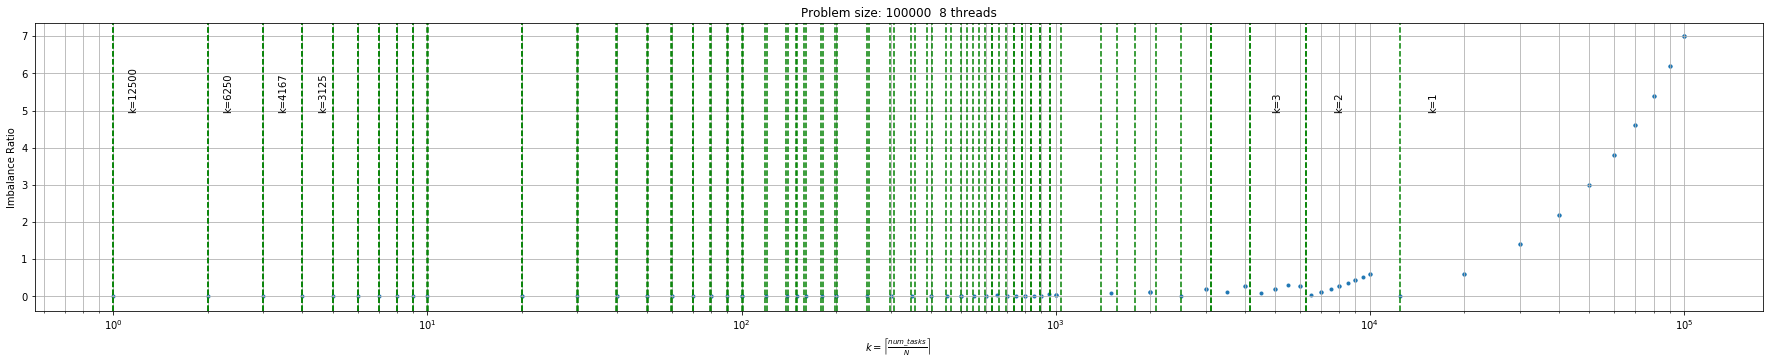
\includegraphics[scale=.25]{images/hpx_for_loop/w_c_all.png}}
	\caption{The imbalance ratio calculated for different grain sizes for $problem\_size=10000$, on 8 cores, where $k=\left\lceil{\frac{num\_{tasks}}{N}}\right \rceil$.}\label{fig38}		
\end{figure}


%\vspace{\baselineskip}	
%\begin{figure}[H]
%	\centering
%	{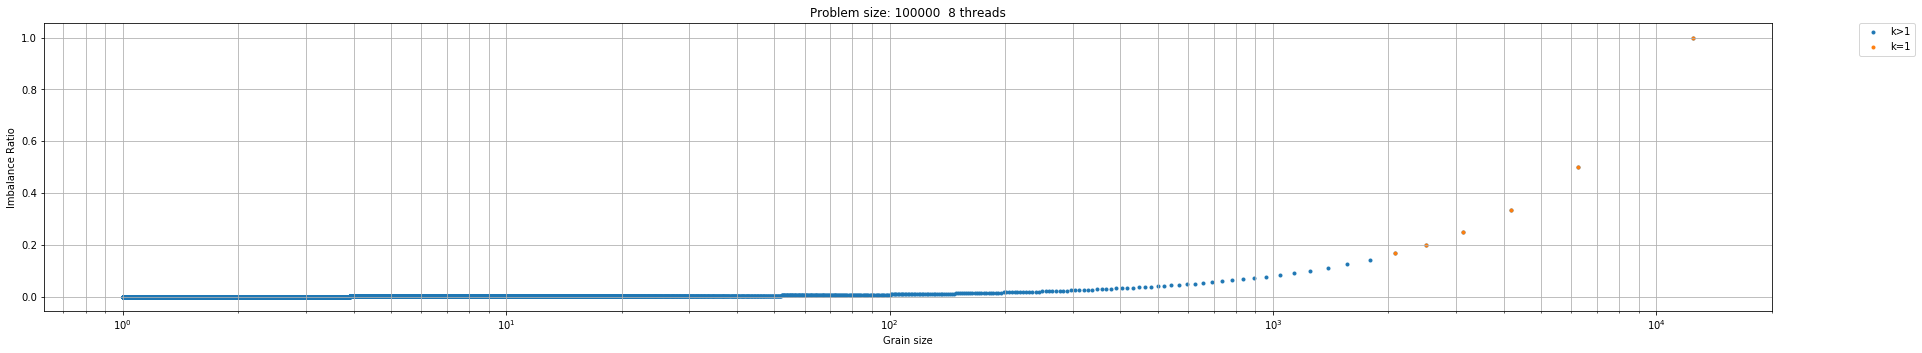
\includegraphics[scale=.45]{images/hpx_for_loop/max_w_c.png}}
%	\caption{The maximum imbalance ratio calculated for different grain sizes for $problem\_size=10000$, on 8 cores, where $k=\left\lceil{\frac{num\_{tasks}}{N}}\right \rceil$.}\label{fig36}		
%\end{figure}

Figure~\ref{fig39} represents the imbalance ratio, along with the ratio of the sequential execution time over execution time(speed-up) against grain size for $problem\_size=10000$, ran on 8 cores.   
As it can be observed, as the $imbalance\_{ratio}$ increases, the speed-up decreases. 

\vspace{\baselineskip}	
\begin{figure}[H]
	\centering
	{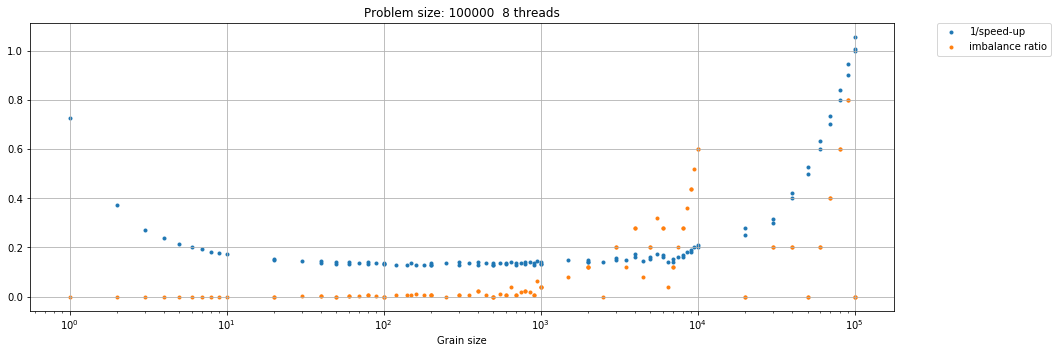
\includegraphics[scale=.3]{images/hpx_for_loop/w_c_speedup.png}}
	\caption{The imbalance ratio calculated for different grain sizes for $problem\_size=10000$, on 8 cores, where $k=\left\lceil{\frac{num\_{tasks}}{N}}\right \rceil$.}\label{fig37}		
\end{figure}


To summarize, as the grain size increases the maximum imbalance in the loads assigned to the cores also increases, and some point on, this imbalance has a significant affect in the execution time. We define a threshold, $\lambda_s$ ($0<\lambda_s<1$), where for $imbalance\_{ratio}$s smaller than this threshold the imbalance effect is not significant. As we get close to this threshold, we are likely to reach the right hand side of the flat region of the bathtub curve of the execution time against grain size. 


We are interested in finding the maximum grain size that would generate a reasonable imbalance ($imbalance\_{ratio}\leq{\lambda_s}$), to make sure we should stay in the flat region of the bathtub curve of execution time against grain size, from load imbalance point of view.  

Formula~\ref{formula14} states that for grain sizes greater than $problem\_{size}$, $imblance\_{ratio}$ increases linearly with grain size from $0$ to $N-1$. While for grain sizes smaller than $problem\_{size}$, the maximum $imbalance\_{ratio}$ depends on $k=\left\lceil{\frac{num\_{tasks}}{N}}\right\rceil$. So, in order to assure $imbalance\_{ratio}$ is smaller than or equal to a threshold ($\lambda_s$), first we search the grain sizes smaller than $\frac{problem\_{size}}{N}$. Since $0<\lambda_s<1$, and $k\geq2$ in this region, there exists a $k$ such that $\frac{1}{k-1}\leq\lambda_s$.    
If there exists a $k_{min}$ (creating an imbalance ratio between $0$ and $\frac{1}{k_{min}-1}$), where $\frac{1}{k_{min}-1}\leq{\lambda_s}$, $\forall k<k_{min}$ maximum value of $imbalance\_{ratio}$ would be greater than $\lambda_s$. So in order to find the grain size that would create maximum $imbalance\_{ratio}$ of $\lambda_s$:



\begin{equation}\label{formula21}
\begin{aligned}
imbalance\_{ratio}\leq{{\lambda_s}}\Rightarrow\\
\frac{1}{k-1}\leq\lambda_s\\
k\geq{1+\frac{1}{\lambda_s}}\\
k_{min}=\left\lceil{1+\frac{1}{\lambda_s}}\right\rceil+1\\
{g}<\frac{problem\_{size}}{(k_{min}-1)\times{N}}\\
g_{max}=\frac{problem\_{size}}{(k_{min}-1)\times{N}}-1=\frac{problem\_{size}}{(1+\left\lceil{\frac{1}{\lambda_s}}\right\rceil)\times{N}}
\end{aligned}
\end{equation}

If $g<g\_{max}$, we can assure that $imbalance\_{ratio}$ never exceeds $\lambda_s$. Since we already found a match at grain sizes smaller than $\frac{problem\_{size}}{N}$, checking the rest of grain sizes would not be necessary.





\begin{lstlisting}[basicstyle=\fontsize{8}{9}\selectfont,float,floatplacement=H,caption= {A simple hpx for\textunderscore{loop} used to study the effect of grain size on the achieved parallelism.}, label={hpx_for_loop}]

///////////////////////////////////////////////////////////////////////////////
void measure_function_futures_for_loop(std::uint64_t count, bool csv, std::uint64_t chunk_size, std::uint64_t iter_length)
{
// start the clock
high_resolution_timer walltime;
hpx::parallel::for_loop(hpx::parallel::execution::par.with(
hpx::parallel::execution::dynamic_chunk_size( chunk_size )),
0, count, [&](std::uint64_t) { worker_timed(iter_length*1000); });
// stop the clock
const double duration = walltime.elapsed();
print_stats("for_loop", "par", "parallel_executor", count, duration, csv);
}

///////////////////////////////////////////////////////////////////////////////
int hpx_main(variables_map& vm)
{
{
const int repetitions = vm["repetitions"].as<int>();
num_threads = hpx::get_num_worker_threads();
const std::uint64_t chunk_size = vm["chunk_size"].as<std::uint64_t>();
const std::uint64_t iter_length = vm["iter_length"].as<std::uint64_t>();
const std::uint64_t count = vm["num_iterations"].as<std::uint64_t>();
bool csv = vm.count("csv") != 0;
if (HPX_UNLIKELY(0 == count))
throw std::logic_error("error: count of 0 futures specified\n");
for (int i = 0; i < repetitions; i++)
{
measure_function_futures_for_loop(count, csv, chunk_size, iter_length);
}
}
return hpx::finalize();
}
///////////////////////////////////////////////////////////////////////////////
inline void worker_timed(std::uint64_t delay_ns)
{
if (delay_ns == 0)
return;
std::uint64_t start = hpx::util::high_resolution_clock::now();
while (true)
{
// Check if we've reached the specified delay.
if ((hpx::util::high_resolution_clock::now() - start) >= delay_ns)
break;chunk
}
}
///////////////////////////////////////////////////////////////////////////////
int main(int argc, char* argv[])
{
// Configure application-specific options.
options_description cmdline("usage: " HPX_APPLICATION_STRING " [options]");
cmdline.add_options()("num_iterations",
value<std::uint64_t>()->default_value(500000),
"number of iterations to invoke")
("repetitions", value<int>()->default_value(1),
"number of repetitions of the full benchmark")
("iter_length",value<std::uint64_t>()->default_value(1), "length of each iteration")
("chunk_size",value<std::uint64_t>()->default_value(1), "chunk size");
// Initialize and run HPX.
return init(cmdline, argc, argv);
}
\end{lstlisting}

\vspace{\baselineskip}
\subsection{Identifying the range of grain size for maximum speedup}
In the previous section, we proposed a method to identify the lower-bound and the upper-bound of the grain sizes for which we observe the minimum execution time. 
Integrating Formula~\ref{formula4} and Formula~\ref{formula21} suggests the following range for maximum speedup:


\begin{equation}\label{formula23}
\begin{aligned}
{\sqrt{\frac{(\frac{\alpha}{N}+\beta\times(N-1))\times{problem\_{size}}}{{\lambda_b}}}}\leq{g}\leq\frac{problem\_{size}}{(1+\left\lceil{\frac{1}{\lambda_s}}\right\rceil)\times{N}}
\end{aligned}
\end{equation}
 
Where $0\leq\lambda_s\leq1$, and $\lambda_b,\lambda_s\ll1$.

In this section we represent the identified range for a number of problem sizes, with different number of cores.


%\vspace{\baselineskip}
%\subsection{Analyzing the Data}
%Throughout these experiments we try to fix or eliminate the factors we believe will affect the execution time as much as possible, study the results, and then introduce one factor to the model and study the behavior of the model. 



\vspace{\baselineskip}
%\subsection{Step 1: Sequential Run}
%In the first step in order to eliminate all the factors related to parallel execution we run the code sequentially for some problem sizes. The obtained result, as shown in Figure~\ref{fig26} demonstrates an overhead that increases as the number of iterations increases.
%
%\begin{figure}
%	\centering
%	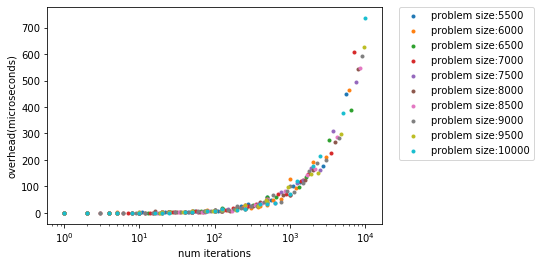
\includegraphics[width=1\linewidth]{images/hpx_for_loop/overheads_seq.png}
%	\caption{The results obtained from running the hpx for loop sequentially}	
%	\label{fig26}
%\end{figure}
\vspace{\baselineskip}
\vspace{\baselineskip}
\vspace{\baselineskip}
\vspace{\baselineskip}
\vspace{\baselineskip}
\vspace{\baselineskip}
\vspace{\baselineskip}
\vspace{\baselineskip}
\vspace{\baselineskip}
\vspace{\baselineskip}
\vspace{\baselineskip}


\subsection{Step 1: Single-task, single-core runs}
At the first step, we look at the cases where only one task has been created, the program is run on only one core. This problem could be assumed to be equivalent to running the same amount of work sequentially with an additional cost of creating just one task. 

\vspace{\baselineskip}
\vspace{\baselineskip}
\vspace{\baselineskip}
\vspace{\baselineskip}
\vspace{\baselineskip}
\vspace{\baselineskip}
\vspace{\baselineskip}
\vspace{\baselineskip}
\vspace{\baselineskip}
\vspace{\baselineskip}
\vspace{\baselineskip}









\subsubsection{Expected Model}
With this assumption we expect the execution time to be summation of the time it takes to perform the total amount of work(\textit{problem\textunderscore{size}}) and the overhead of creating one HPX task($\alpha$). Formula~\ref{chunk1} shows the expected formula.

\begin{equation}\label{chunk1}
execution\:\:time = \alpha + problem\:\:size
\end{equation}  

\vspace{\baselineskip}
\subsubsection{Original Data}
In order to check our proposed model for this simplified problem, we collected data from running the program, setting the \textit{chunk\textunderscore{size}} to 1, \textit{num\textunderscore{iterations}} to 1, and changing the \textit{iter\textunderscore{length}} from 1 to 10,000,000. 




%To summarize, knowing the grain size, we are expecting the execution time in a many-task runtime system to be mainly affected by these factors, the overhead of creating one task($\alpha$), the number of cores that are actually doing the work($M$), the sequential execution time($t_s$), and finally the portion of the program that could actually be parallelized($\gamma$). 
%
%If we try to integrate these information into a formula, we would expect the relation between execution time($t$) and number of tasks($n_t$) as follows:
%\begin{equation}\label{new1}
%t=\frac{\alpha{n_t}+t_s}{M}+\gamma
%\end{equation}
%
%which could be decomposed into these two equations:
%
%
%Now we use this function to find the best three parameters $\alpha$, $t_s$, and $\gamma$ so that the collected data would fit this model. For this purpose we used the \textit{curve\textunderscore{fit}} package from \textit{SciPy} library in \textit{python}.
%
%In order to make Equation~\ref{new1} differentiable, we used the softplus function(Equation~\ref{softplus1}) to represent $M$ based on $n_t$.
%\begin{equation}\label{softplus1}
%f(x)=Ln(1+e^x)
%\end{equation}
%
%Which results in Equation~\ref{soft_plus1}:
%\begin{equation}\label{soft_plus1}
%t=\frac{\alpha{n_t}+t_s}{(N-1)-Ln(1+(e^{N-1}-1)e^{-n_t})}+\gamma
%\end{equation}




\vspace{\baselineskip}